\begin{frame}
  \frametitle{Express Parallel Algo independent of processors}
  \begin{figure}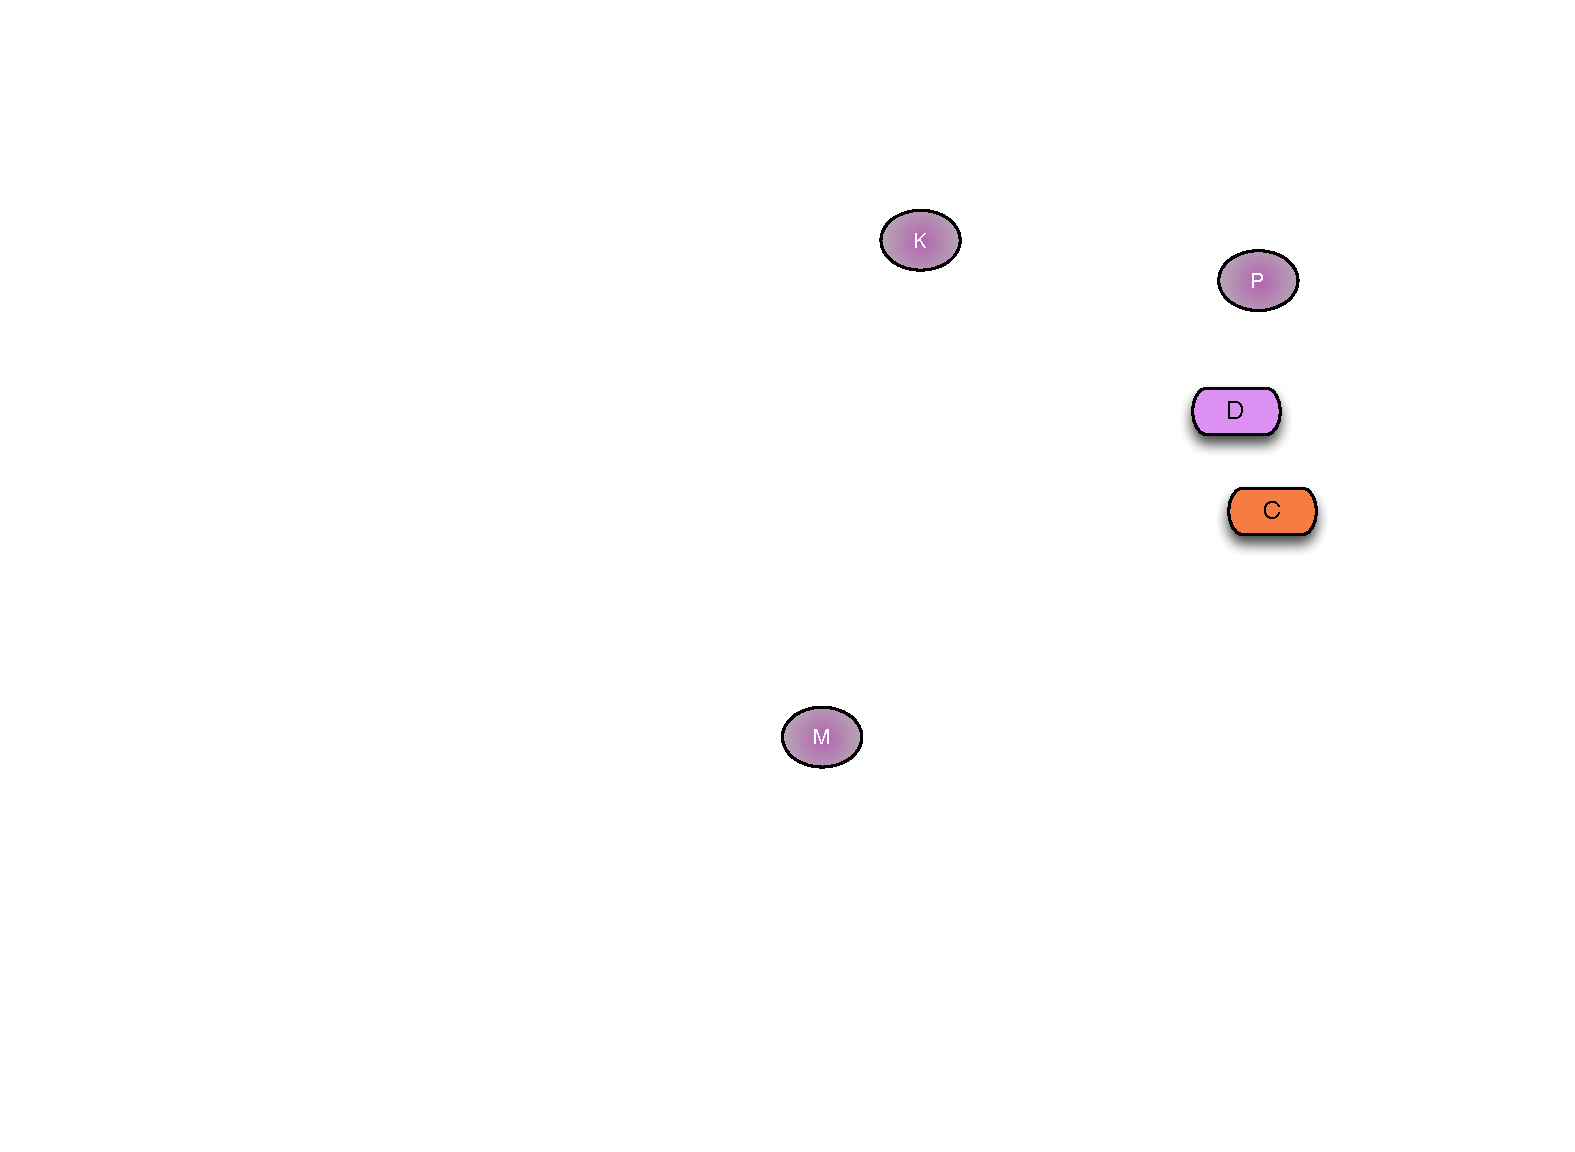
\includegraphics[width=0.9\textwidth]{../figures/progmodel/01-objects-for-algo.pdf}\end{figure}
\end{frame}


\begin{frame}
  \frametitle{Data Decomposition via Collections of Objects}
  \begin{figure}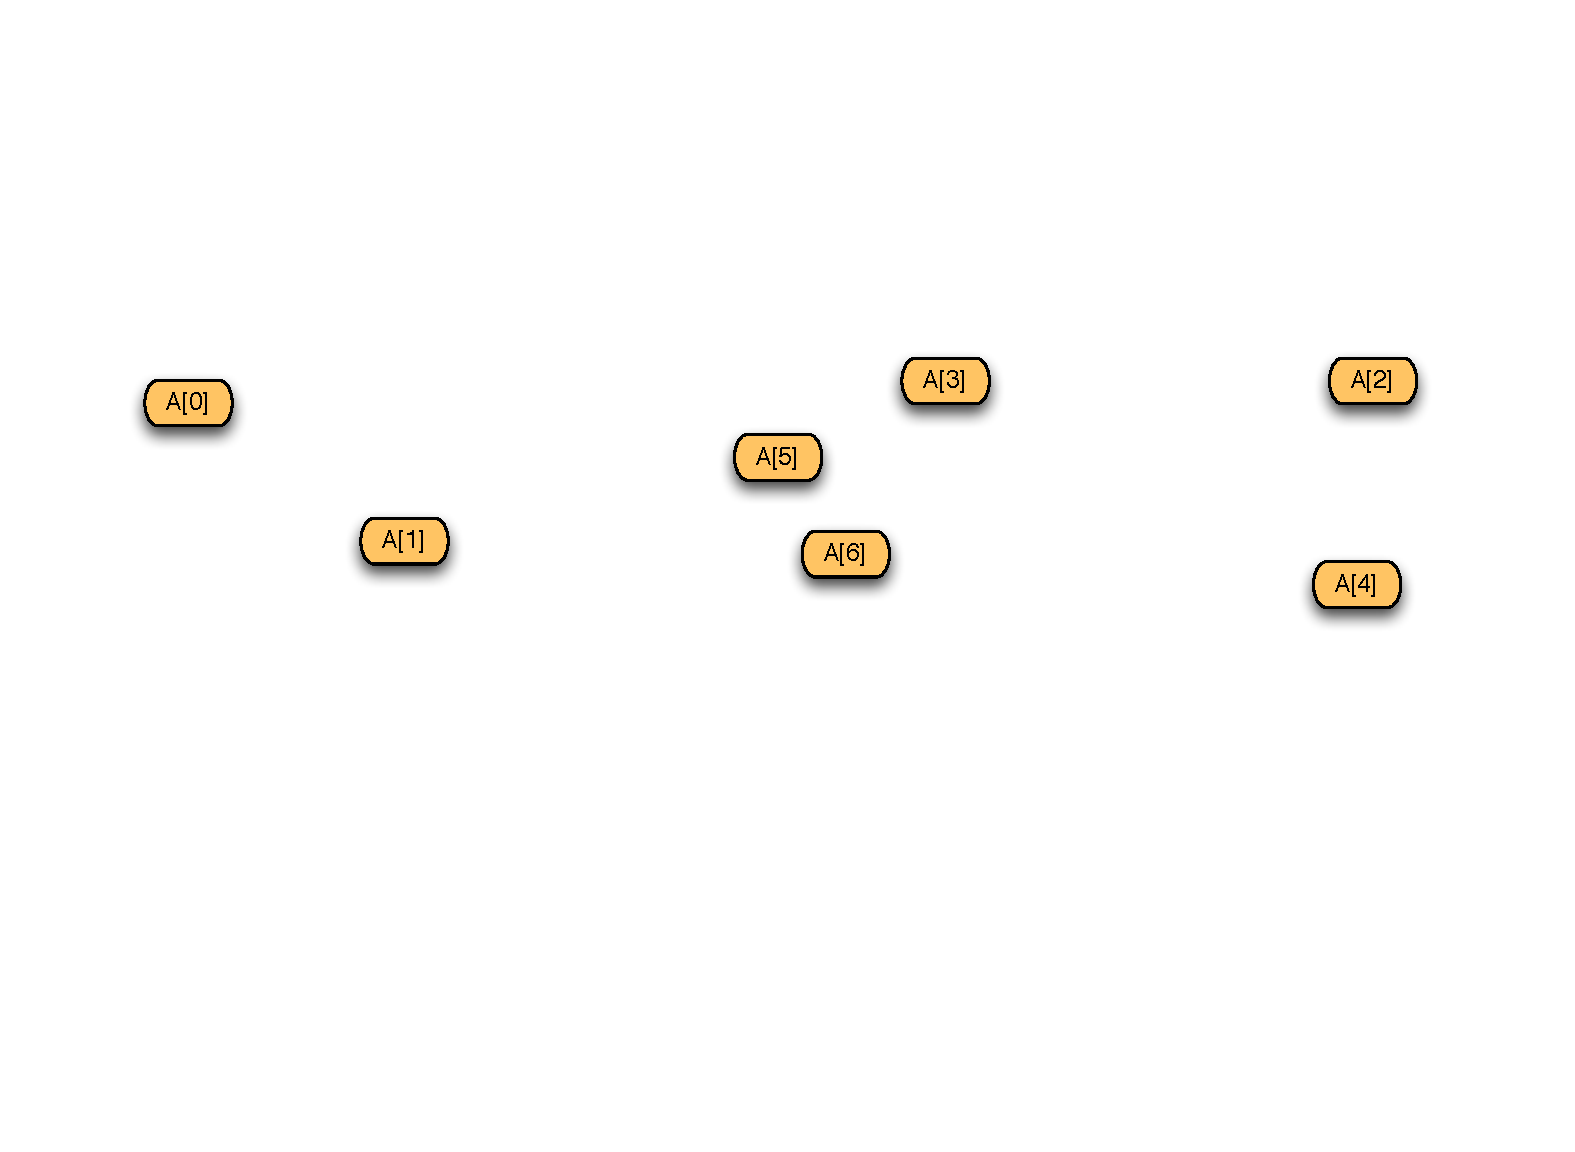
\includegraphics[width=0.9\textwidth]{../figures/progmodel/02-data-decomp-via-arrays.pdf}\end{figure}
\end{frame}


\begin{frame}
  \frametitle{Multiple data parallel control flows}
  \begin{figure}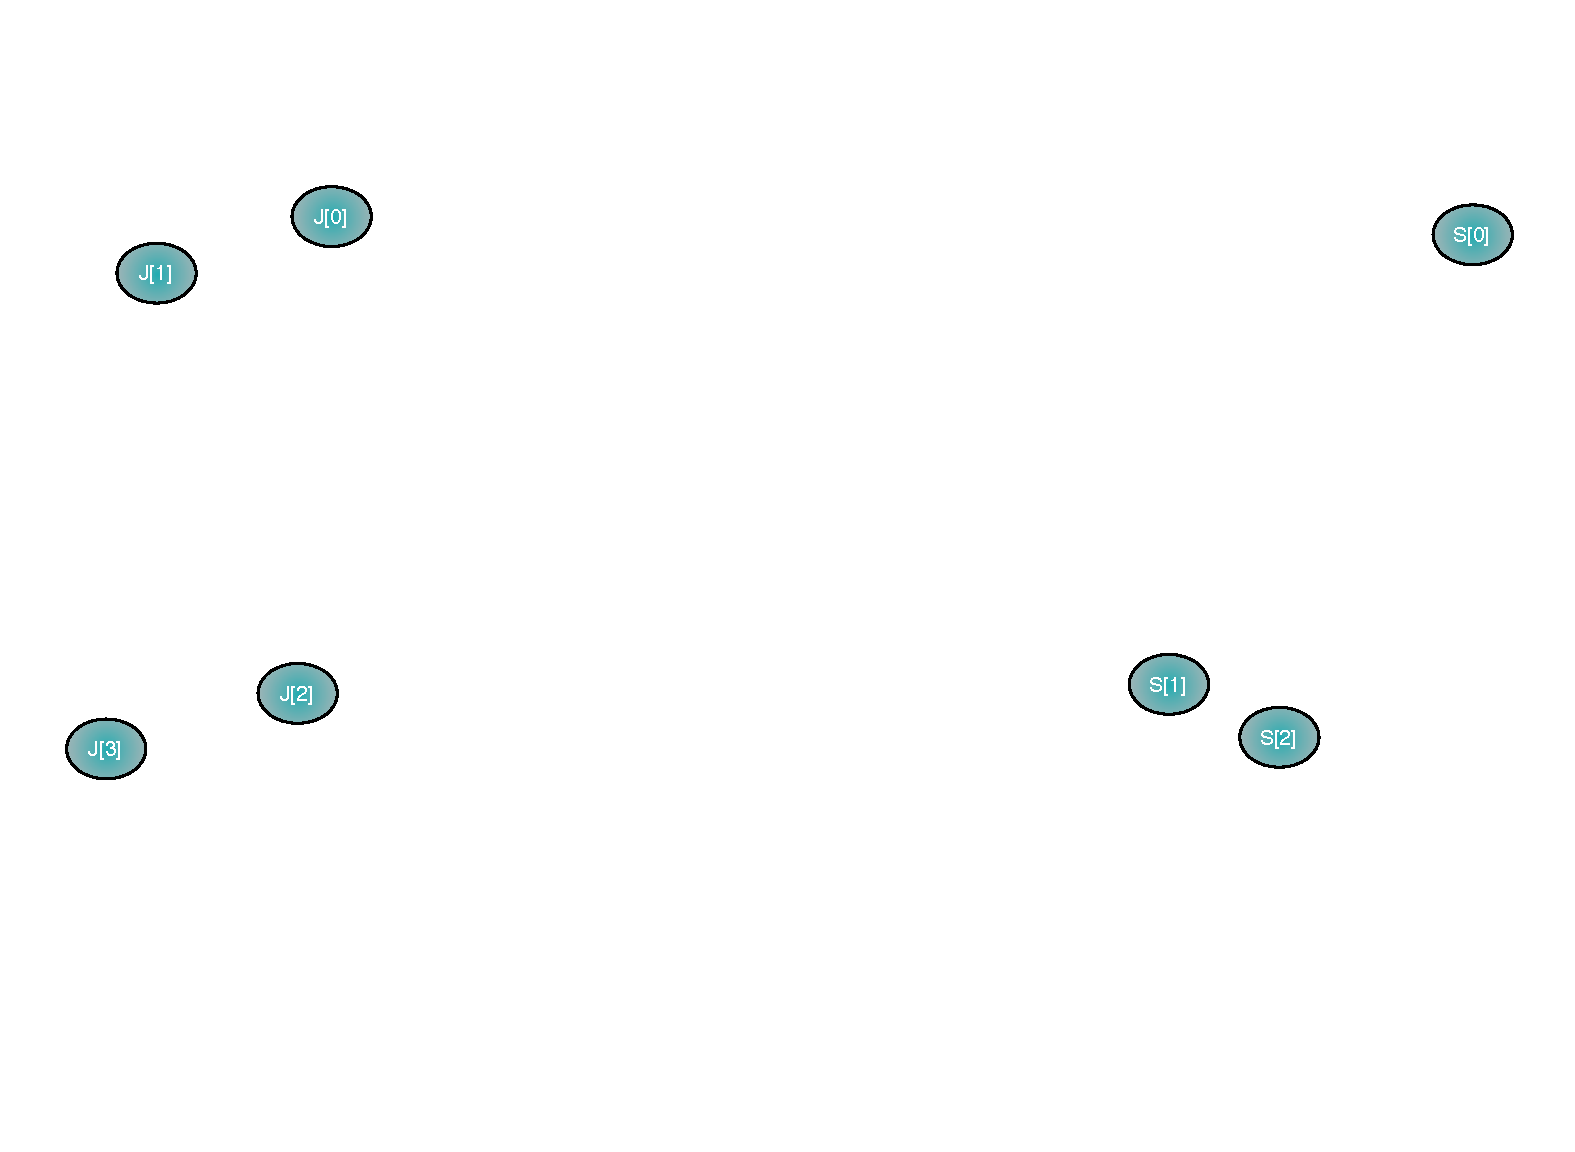
\includegraphics[width=0.9\textwidth]{../figures/progmodel/03-many-data-parallel-arrays.pdf}\end{figure}
\end{frame}


\begin{frame}
  \frametitle{Decompose parallel functionality into interacting classes}
  \begin{figure}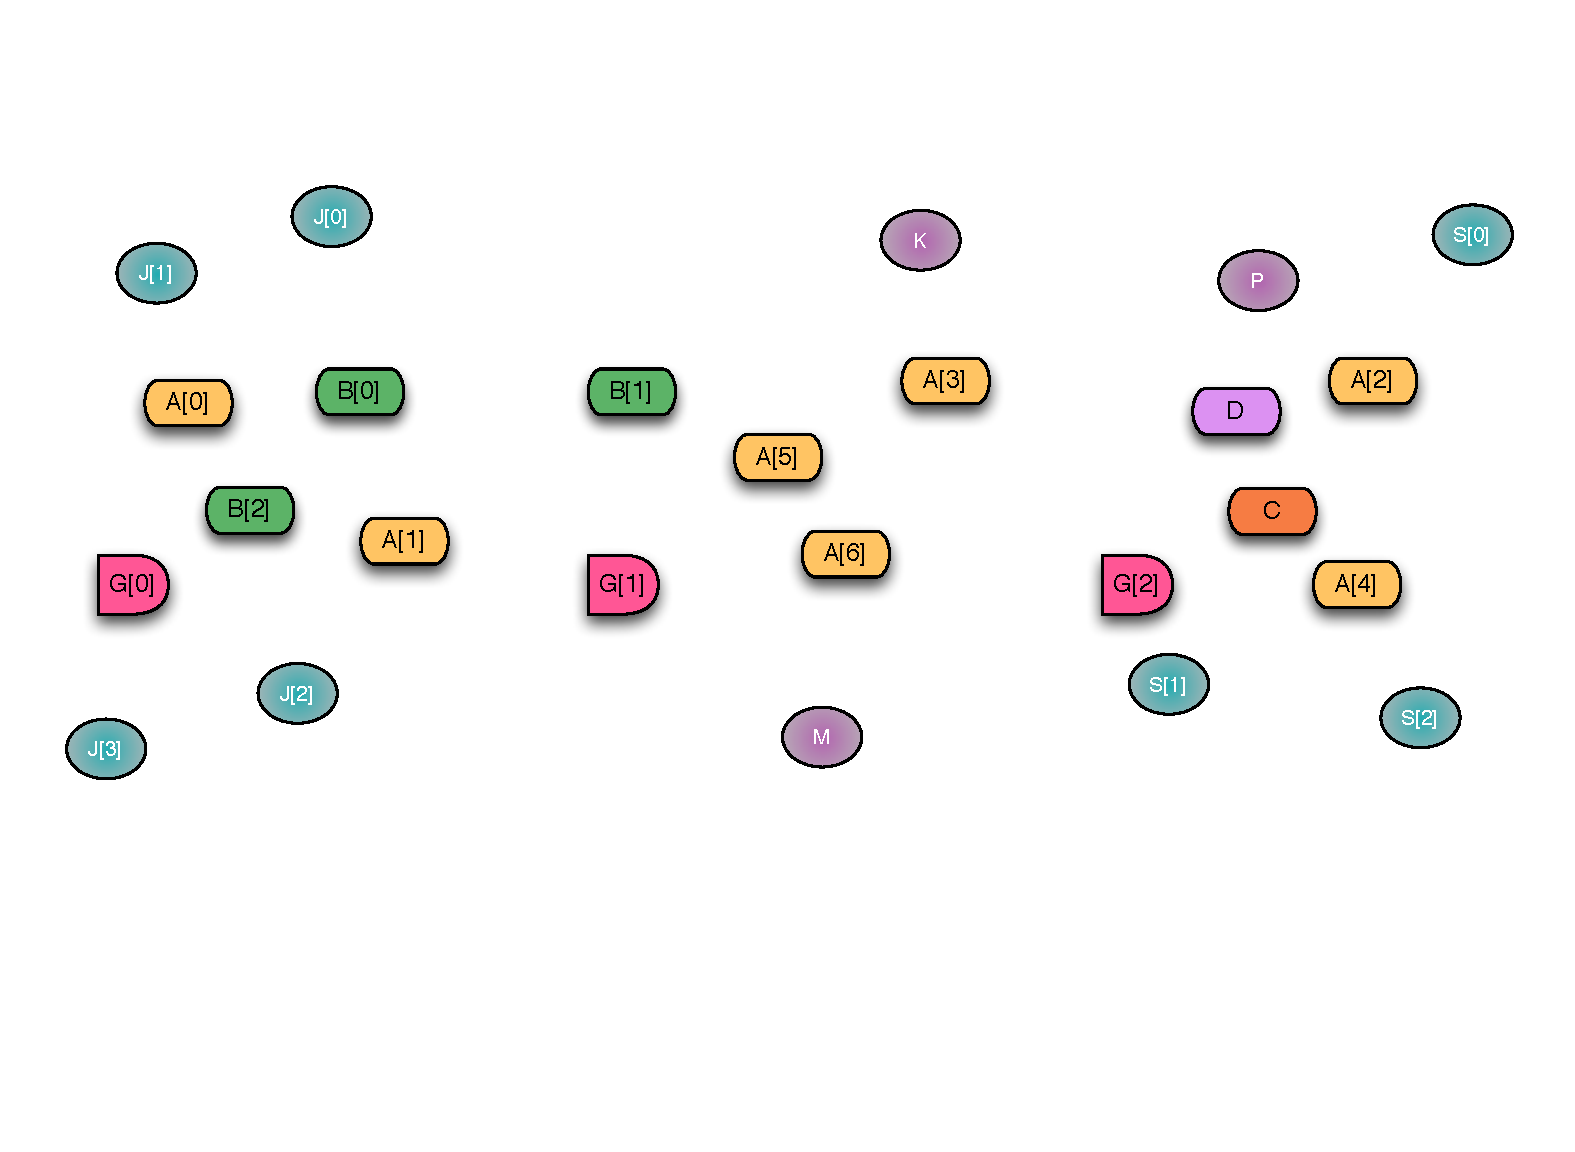
\includegraphics[width=0.9\textwidth]{../figures/progmodel/04-func-decomp-via-classes.pdf}\end{figure}
\end{frame}


\begin{frame}
  \frametitle{
    \only<1>{Parallelism requires distributing objects across processors}
    \only<2>{However, do not burden programmer with this view}
  }
  \begin{figure}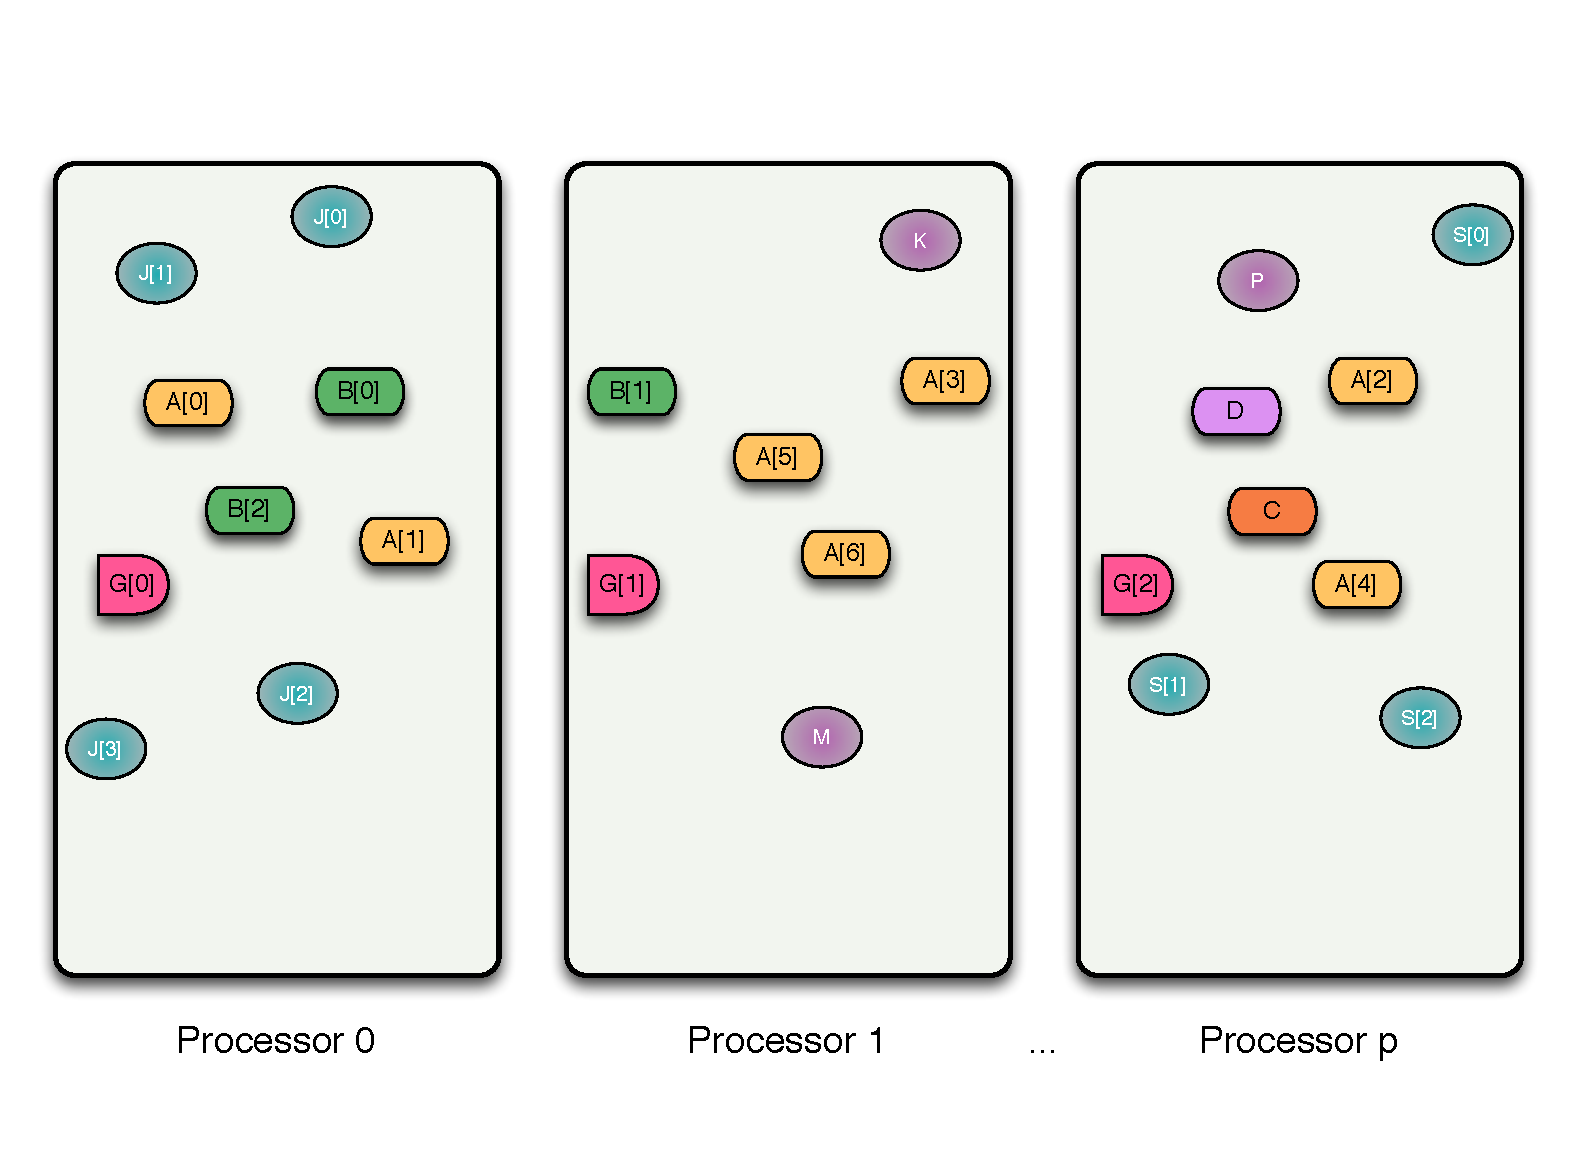
\includegraphics[width=0.9\textwidth]{../figures/progmodel/05-objects-sys-view.pdf}\end{figure}
\end{frame}


\begin{frame}
  \frametitle{
    \only<1>{Elevate some objects to global visibility}
    \only<2>{Addressing objects is independent of location}
  }
  \begin{figure}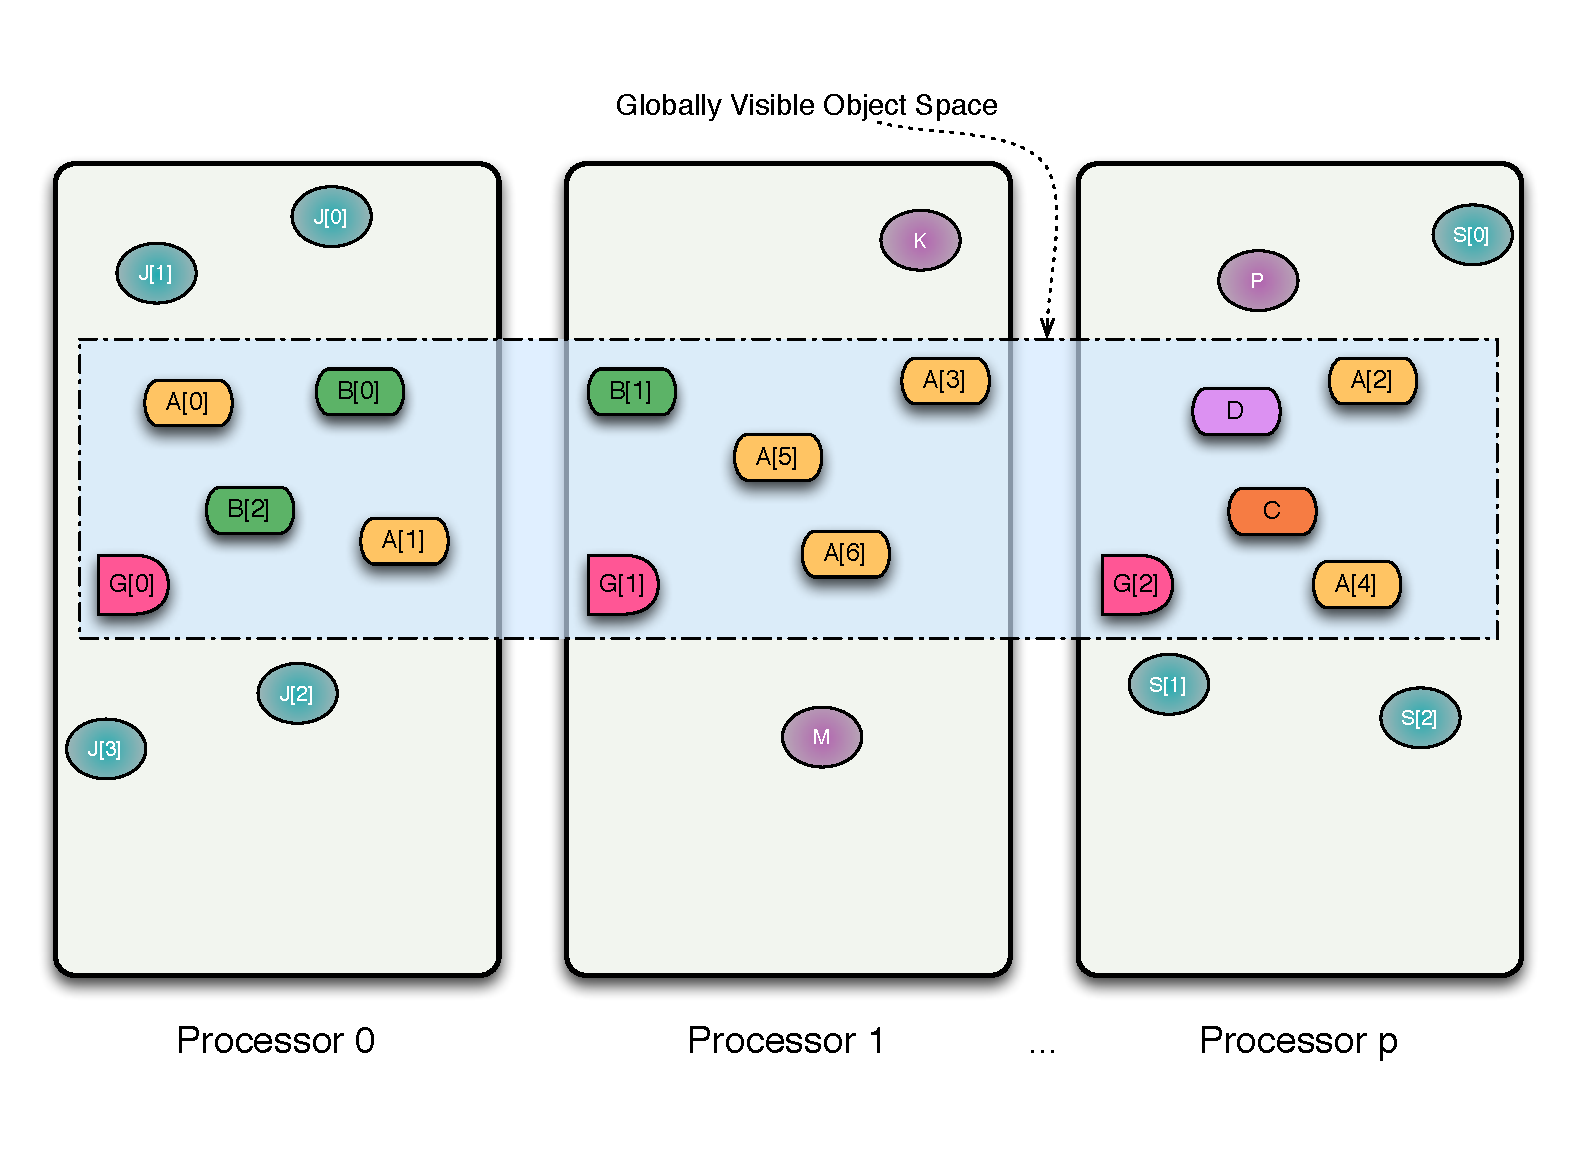
\includegraphics[width=0.9\textwidth]{../figures/progmodel/06-elevate-obj-2-global-space.pdf}\end{figure}
\end{frame}


\begin{frame}
    class / object - fundamental unit of state natural to parallel algo\\
    method - fundamental unit of execution in parallel algo\\
    express parallel algo interactions via methods or function calls
\end{frame}


\begin{frame}
  \frametitle{Objects interact via methods}
  \begin{figure}
    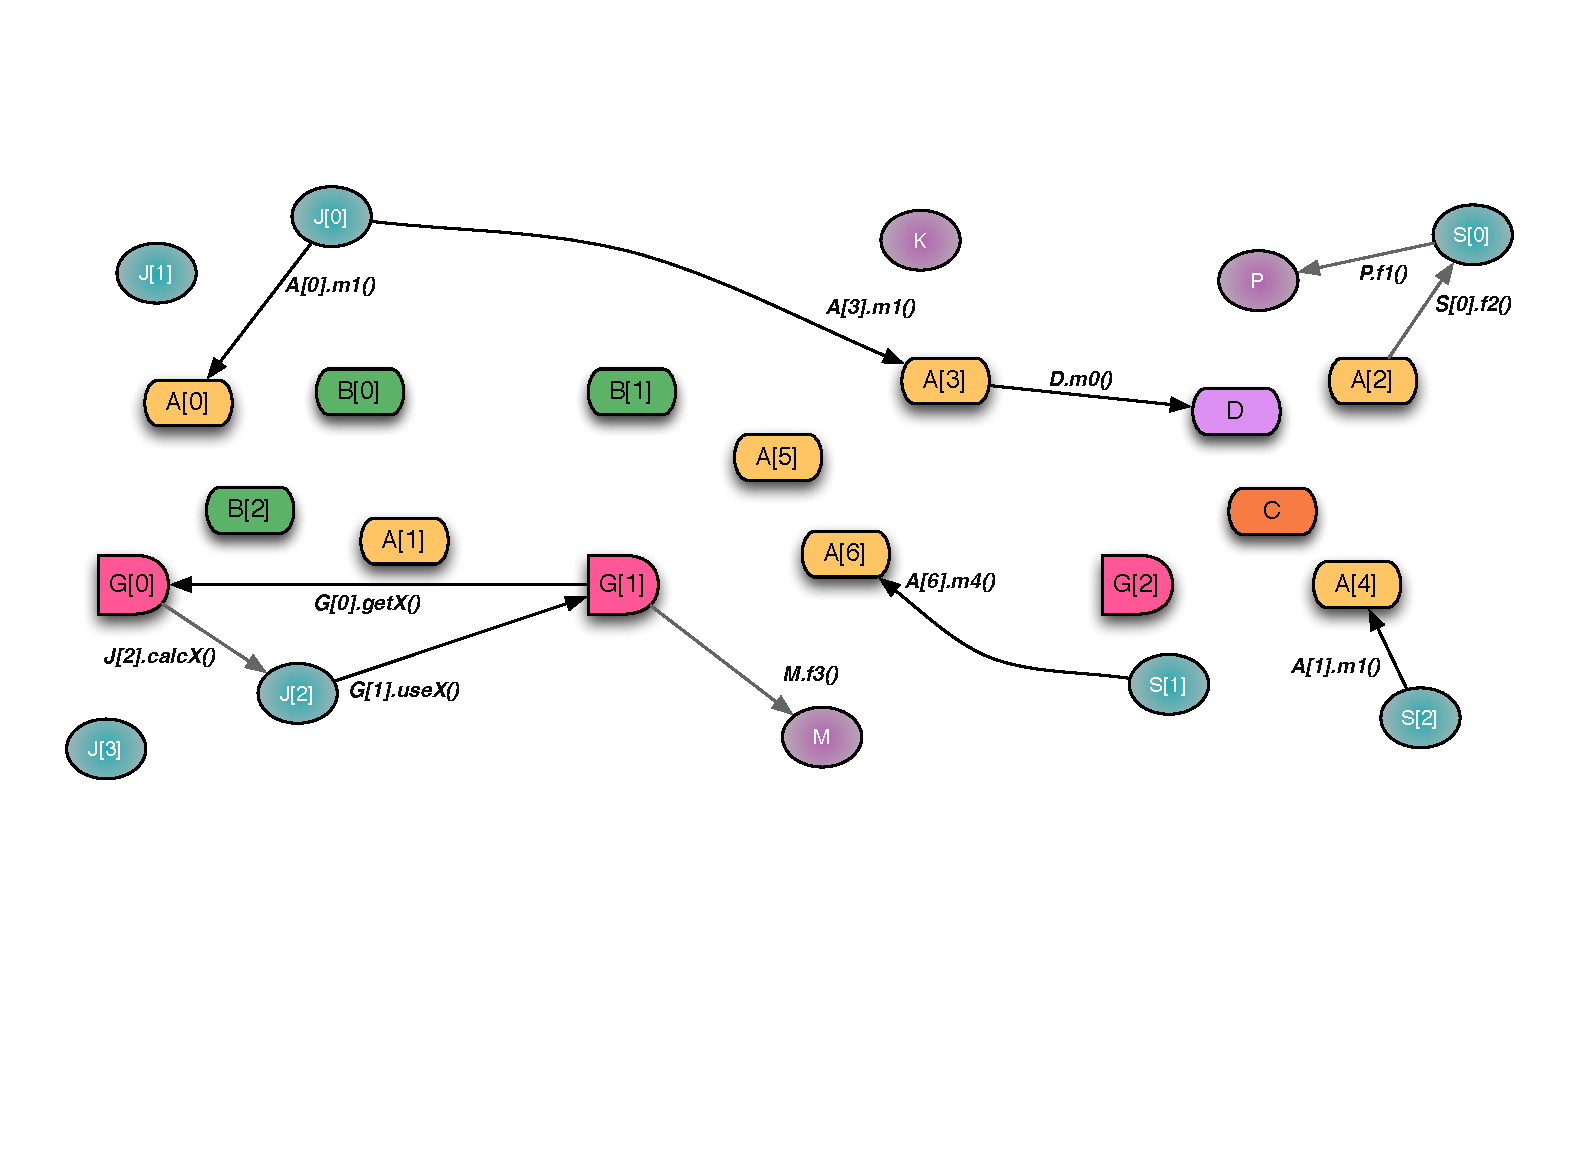
\includegraphics[width=0.9\textwidth]{../figures/progmodel/07-algo-via-objects-methods.pdf}
  \end{figure}
\end{frame}


